% !TeX spellcheck = en_US
\documentclass[
    10pt,
    A4,
    polish,
    draft = false,
    twoside = false,
]{article}

\usepackage{curriculum-vitae}
\usepackage{tikz}
\usepackage{graphicx}
\usetikzlibrary{calc}
\usepackage{fancyhdr}

\cfoot{\tiny{© Wyrażam zgodę na przetwarzanie moich danych osobowych w celu rekrutacji zgodnie z art. 6 ust. 1 lit. a Rozporządzenia Parlamentu Europejskiego i Rady (UE) 2016/679 z dnia 27 kwietnia 2016 r. w sprawie ochrony osób fizycznych w związku z przetwarzaniem danych osobowych i w sprawie swobodnego przepływu takich danych oraz uchylenia dyrektywy 95/46/WE (ogólne rozporządzenie o ochronie danych)}}
\begin{document}
	%	Basic information	
	\setname{Piotr}{Kornaszewski}
	\setaddress{Siadło Górne 8 / 72-001 Kołbaskowo}
	\setmobile{(+48) 500 793 323}
	\setmail{kornaszewski.piotr@wp.pl}
    \setgithub{\href{https://github.com/Kanekiop1}{ Github}}
    \setlinkedin{\href{https://www.linkedin.com/in/piotr-kornaszewski-783420158/}{Linkedin}}

	%---------------------------------------------------------------------------------------
	%	Title + Contact
	%----------------------------------------------------------------------------------------
	\cvtitle{Curriculum Vitae}
	
	\begin{tikzpicture}[remember picture,overlay]
    \node[anchor=south west,inner sep=0pt, scale=0.14] at ($(current page.south west)+(15.65cm,23.4cm)$) {
     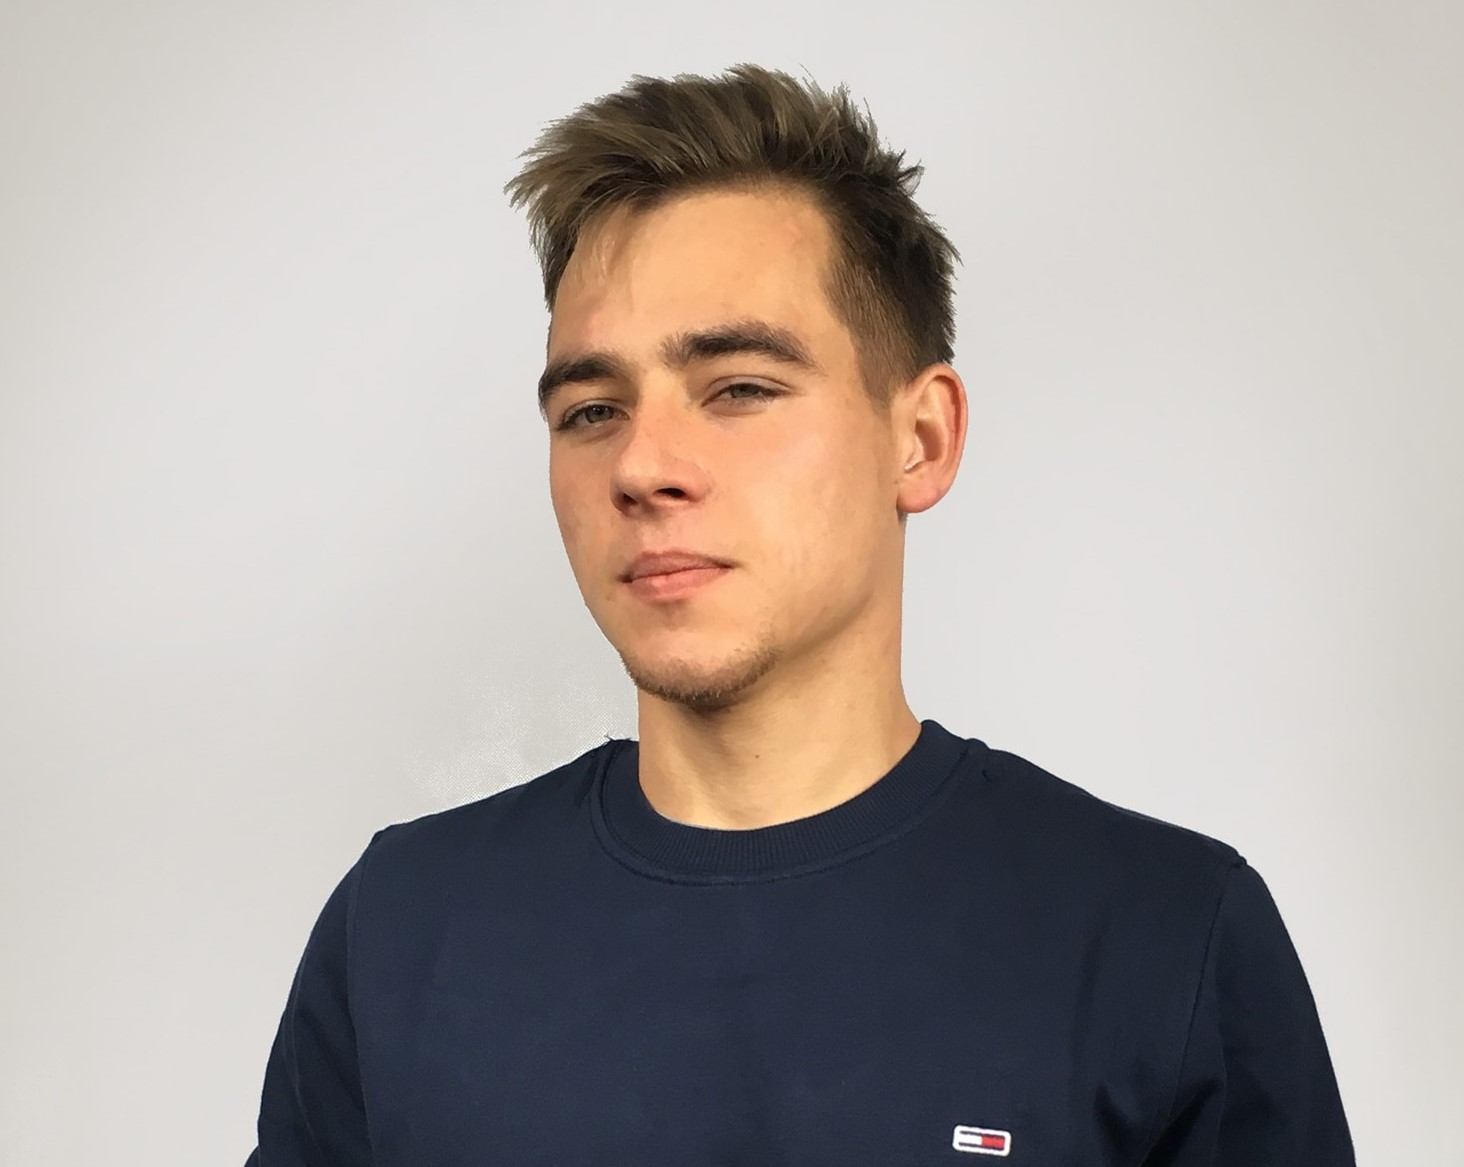
\includegraphics{cv.jpg}
     };
    \end{tikzpicture}
	\hspace{8pt}

	%---------------------------------------------------------------------------------------
	%	Summary / Objectives
	%----------------------------------------------------------------------------------------
    \cvSection{O mnie}	
    \CVTextBlock{ Zmotywowany inżynier automatyki i robotyki posiadający blisko trzy i pół roku doświadczenia w zakresie sprzętu i oprogramowania. Od początku w dziedzinie awioniki UTM i UAV, w szczególności dronów. Zawsze szukający nowych wyzwań i poszerzania wiedzy.}
	%---------------------------------------------------------------------------------------
	%	Current Position
	%----------------------------------------------------------------------------------------
%	\cvSection{Current Position}
	%---------------------------------------------------------------------------------------
	%	Education
	%----------------------------------------------------------------------------------------
	
	\cvSection{Wykształcenie}
	\CVBlockWithTime{Zachodniopomorski Uniwersytet technologiczny w Szczecinie}{2/2020 - 9/2021}
	{Wydział Elektryczny}{Szczecin, Polska}
	{\textbf{Kierunek} Automatyka i Robotyka, Studia Magisterskie}
    \CVBlockWithTime{Zachodniopomorski Uniwersytet technologiczny w Szczecinie}{9/2016 - 2/2020}
	{Wydział Elektryczny}{Szczecin, Polska}
	{\textbf{Kierunek} Automatyka i Robotyka, Studia Inżynierskie}
	%---------------------------------------------------------------------------------------
	%	Experience (Research and Industry)
	%----------------------------------------------------------------------------------------
%	\cvSection{Experience (Research \& Industry)}
	\cvSection{Doświadczenie}
	\CVBlockWithTime{Tester sprzętu i oprogramowania}{1/2022 - obecnie}{Aerobits Sp. z o.o.}{Szczecin, Polska}
	{Pisanie testów sprzętowych z wykorzystaniem jezyka Python, Linux/Bash, walidacja oprogramowania oraz sporządzanie dokumentacji technicznej}	
    \CVBlockWithTime{Inżynier Elektronik}{8/2021 - 12/2021}{Aerobits Sp. z o.o.}{Szczecin, Polska}
	{Montaż prototypowych modułów radiowych, diagnostyka uszkodzeń oraz sporządzanie dokumentacji technicznej} 
    \CVBlockWithTime{Technik Elektronik}{7/2019 - 8/2021}{Aerobits Sp. z o.o.}{Szczecin, Polska}
	{Montaż, naprawa modułów radiowych oraz sporządzanie dokumentacji technicznej}

	%---------------------------------------------------------------------------------------
	%	Skills
	%----------------------------------------------------------------------------------------
	\cvSection{Umiejętności}
	\tab \begin{tabular}{r p{0.7\textwidth}}
		\texttt{\large Języki programowania} & \textbf{Python} 
		   - pisanie bloków testujących sprzęt z wykorzystaniem komunikacji UART/USB, oraz testy oprogramowania,
            aplikacje obsługujące bazy danych (DB, SQLite), 
            wyciąganie tabel ze stron www i obróbka danych, \newline 
        \textbf{Github/yml} - tworzenie oraz utrzymywanie CI zgodnie z wytycznymi projektów, \newline
        \textbf{Latex} - sporządzanie dokumentacji technicznej, jak i dokumentacji sprzedażowej, \newline
        \textbf{matlab} - korzystanie z global optymalization toolbox w celu generowania trajektorii robota mobilnego, \newline
        \textbf{C} - proste programy obsługujące Atmege32 z wykorzystaniem sensorów, \newline
        \textbf{C\#} - aplikacja obiektowa do obsługi manipulatora przemysłowego z wykorzystaniem transmisji RS232, \newline
        \textbf{Linux\textbackslash Bash} - proste skrypty systemowe wykorzystujące funkcjonalności aplikacji Python \\
		\texttt{\large Środowiska \& Narzędzia} & Git \cvContactSep Windows \cvContactSep Linux \cvContactSep Matlab \cvContactSep Jupyter \cvContactSep VSCode \cvContactSep Texstudio \\
		\texttt{\large Języki} & \textbf{Natywny:} Polski \cvContactSep \textbf{Obce:} Angielski (B1/B2)  \\
        \texttt{\large Miękkie} & Pracowitość \cvContactSep Sumienność \cvContactSep Praca zespołowa  \\
	\end{tabular}\\~\\
	
	%----------------------------------------------------------------------------------------
\end{document}
